\documentclass[11pt]{article}
\usepackage{graphicx}
\usepackage{units}

\begin{document}
\title{Lesson 10 Homework}
\author{Colt Bradley}
\date{}
\maketitle


\section{Part 1}
The first part of this homework assignment was relatively simple. Using the given equation, I used the $logspace$ command to create a logarithmically distributed list of values from $10^{-1}$ to $10^7$. I then evaluated the equation (\ref{dragcoefficent}) for each of these values and plotted the solution. 

\begin{equation}
C_d (R_e) = \frac{24}{R_e}+\frac{2.6 (\frac{R_e}{5})}{1+(\frac{R_e}{5})^{1.52}}+\frac{0.411 (\frac{R_e}{263000})^{-7.94}}{1+(\frac{R_e}{263000})^{-8.00}}+\frac{(R_e)^{0.80}}{461000} \label{dragcoefficent}
\end{equation}

\begin{figure}[ht]
\centering
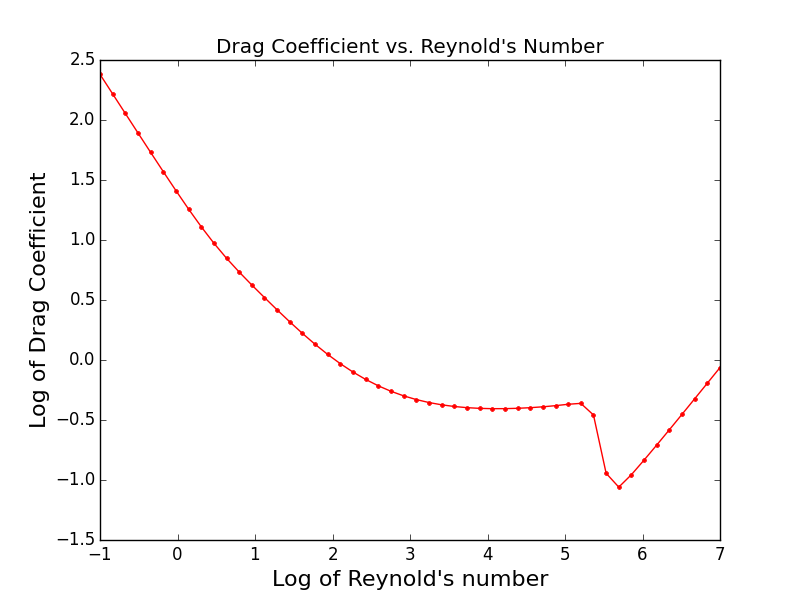
\includegraphics[scale=.5]{cdvsreplot.png}
\end{figure}

Notice we start getting strange results when $R_e = 10^6$, which is the upper limit to where this function is valid. 

\section{Part 2}
Next, I needed to solve the shotgun pellet example. The calculation of the drag coefficient and Reynolds number will have to be included in the loop since they depend on velocity. I use the second order Runge-Kutta method to solve as written in the instructions, and add two calculations of the drag coefficient and Reynolds number, one before the first step and the next before the second step. 


\begin{figure}[ht]
\centering
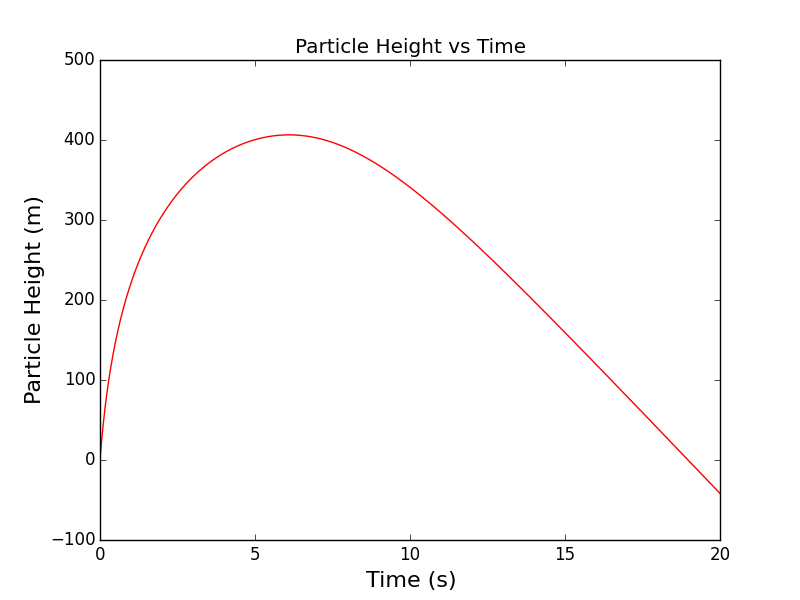
\includegraphics[scale=.4]{heightplot.png}
\end{figure}

\begin{figure}[ht]
\centering
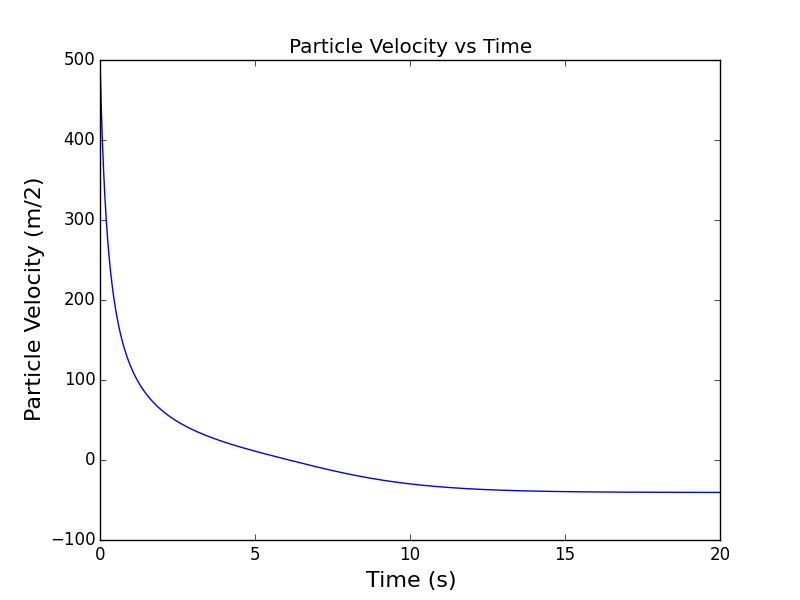
\includegraphics[scale=.4]{velocityplot.png}
\end{figure}

We can tell from these graphs that the maximum height is around $400m$, and the particle hits zero at around $18s$ with a velocity of about $-30 \nicefrac{m}{s}$

\section{Code}

\begin{verbatim}
#Colt Bradley
#2.22.16
#Lesson 10

#import modules
import numpy as n
import pylab as p

#create our logspace
r_e = n.logspace(-1,7)
c_d = []

#create loop
for i in r_e:
    c = (24/i)+((2.6*(i/5.))/(1+(i/5.)**1.52))+ \
    ((.411*(i/263000)**(-7.94))/(1+(i/263000)**(-8.)))+(i**(.8)/461000.)
    c_d.append(c)

#Plot log-log plot
r_e = n.log10(r_e)
c_d = n.log10(c_d)

p.close()
p.plot(r_e,c_d,"r.")
p.plot(r_e,c_d,"r")
p.title("Drag Coefficient vs. Reynold's Number")
p.xlabel("Log of Reynold's number", fontsize = 16)
p.ylabel("Log of Drag Coefficient",fontsize = 16)
p.show()
p.savefig("cdvsreplot.png")


########################################################################3
#########################################################################
#exercise 2
###########################################################################


#define Values
m = .00104
D = .00559
v0 = 500.
rho = 1.28
mu = .0000183

r_e1 = rho*v0*D/mu
#checks if in the apropriate range, if True then it is
print r_e1
print r_e1<10**6

#RK2 method
#define values, using some of above values
v = v0
y0 = 0
y = y0
g = 9.8
A = ((D/2)**2)*n.pi
tf = 20.
ts = 10000
dt = tf/ts
Y = []
V = []
time = []
t = 0

for i in range(0, ts):
    #define reynolds number, drag coefficient for first step
    r_e2 = rho*abs(v)*D/mu
    c_d1 = (24/r_e2)+((2.6*(r_e2/5.))/(1+(r_e2/5.)**1.52))+ \
    ((.411*(r_e2/263000)**(-7.94))/(1+(r_e2/263000)**(-8.)))+ \
    (r_e2**(.8)/461000.)
    
    #do first step
    y1 = y + v*dt/2
    v1 = v + (-g - ((rho*A*abs(v)*c_d1*v)/(2*m)))*dt/2
    
    #define reynolds number, drag coefficent for second step
    r_e3 = rho*abs(v1)*D/mu
    c_d2 = (24/r_e3)+((2.6*(r_e3/5.))/(1+(r_e3/5.)**1.52))+ \
    ((.411*(r_e3/263000)**(-7.94))/(1+(r_e3/263000)**(-8.)))+ \
    (r_e3**(.8)/461000.)
    
    #do second step
    y = y + v1*dt
    v = v + (-g - ((rho*A*abs(v1)*c_d2*v1)/(2*m)))*dt
    
    #interate values and append solutions to a list
    t = t +dt
    V.append(v)
    Y.append(y)
    time.append(t)
    
#create and save plot for the height
p.close()
p.plot(time,Y,"r")
p.title("Particle Height vs Time")
p.ylabel("Particle Height (m)", fontsize = 16)
p.xlabel("Time (s)",fontsize = 16)
p.show()
p.savefig("heightplot.png")

#create and save plot for velocity
p.close()
p.plot(time,V,0,"r")
p.title("Particle Velocity vs Time")
p.ylabel("Particle Velocity (m/2)", fontsize = 16)
p.xlabel("Time (s)",fontsize = 16)
p.show()
p.savefig("velocityplot.png")


\end{verbatim}


\end{document}